\documentclass[12pt,a4paper]{article}
\usepackage{times}
\usepackage{durhampaper}
\usepackage{harvard}
\usepackage{graphicx}

\citationmode{abbr}
\bibliographystyle{agsm}

\title{User Interaction Discovery in Virtual Environments}
\student{L.A. Sutton}
\supervisor{W. Li}
\degree{BSc. Natural Science}

\date{}

\begin{document}

\maketitle

\begin{abstract}

{\bf Context/Background}
In the past 20 years the number of mediated interactions between people has massively increased, mainly though virtual environments; this includes social networks, online games and messaging systems. While there have been previous attempts to visualise these environments, particularly social networks, these have almost exclusively focused on the static relationships between people inside these networks rather than the interactions themselves and also have not taken into account the many different ways in which people can interact simultaneously (mode of interaction).

{\bf Aims}
The aim of the project is to apply what has been discovered in the visualisation and clustering of static pictures of networks and apply this to a dynamic system:  Firstly to produce an effective way of modelling and visualising the interactions taking place in the environments given above, then to use this model and visualisation to discover clustering of these interactions. On top of this I will then be build a way of examining how this changes over time which will include a quantitative output applicable to solving real-world problems.

{\bf Method}
Research will be carried out on existing systems and available literature in order to determine previous approaches and best practices for the visualisation of interactions. Experiments will be made with various algorithms to characterise the clustering and finally research will be conducted into problems to which data from this system could be applied. This will then be used to create a series of prototypes leading to a final solution.

{\bf Proposed Solution}
A system for modelling and visualising multiple modes of interaction will be implemented and a an underlying model will be developed. The system will be configurable and will be able to identify clustering of interactions within the model as well as the changes of this clustering over time. The system will also then be able to provide a meaningful quantitative output to help in the solution of a suitable problem.

\end{abstract}

\begin{keywords}
user interaction; virtual environment; visualisation; clustering
\end{keywords}

\section{Introduction}

\subsection{Project Description and Purpose}
This project is to be an investigation into the ability to visualise user interactions in virtual environments and changes in their clustering over time. This will be done by applying research into visualisation and clustering of static networks of relationships. It will then be seen if the knowledge gained has any real-world application.

\subsubsection{Virtual Environments}
I will take virtual environments to mean any environment in which users interact using a network of electronic devices. This broad definition will include three main areas:
\begin{description}
\item[Social Networks] This includes Facebook and others where users will be mutually linked with others to create a network. Users are able interact in ways such as writing public messages, uploading photos in which others are present (tagged) and by viewing the photos and messages of others.
\item[Online Games] Many games for example World of Warcraft take place in a three dimensional virtual environment in which users are free to move about and interact within this space. These users will then be able to interact by simply seeing one another, by writing messages visible to those within a certain distance or by working cooperatively to complete a task.
\item[Messaging Systems] I use this to include other systems in which users explicitly send each other either visual, audible or by text. This includes for example email which allows users to interact with one or many others by text or VoIP applications such as Skype allowing users to interact in any of those ways with one or more others.
\end{description}

Inferring social networks from areas such as these has been the subject of significant previous research previous research. Networks of social interaction have been produced from a history of email correspondence within an organisation \cite{fisher2004social}. Here as well other relevant ideas are explored such as the privacy implications of collecting data on a large scale and the ability to reconstruct the whole graph from only partial data. The same has also been achieved using the transcript of an internet relay chat \cite{mutton2004inferring} again struggling with the problem of reconstructing a complete graph from partial data. It is then further shown that the same method including the temporal decay of relationships can be applied to other sources of relationship information involving over time.

%check this citation
The evolution of social networks over time has also been a popular area of research; particularly the presence of homophily \cite{adamic2003friends}; the idea that people on social networks tend to associate with people who are similar to themselves in terms of factors such as age and political views. Work has also been completed on the behaviours of users within a social network and the ways in which interactions can spread behaviour across networks of people represented as graphs. It has been suggested that this can be explained using a virus like model \cite{centola2010spread} in which users pass between susceptible, infected and recovered states, analogous to a computer or real virus.

\subsubsection{Interactions}
I will refer to the wide variety of ways in which users can interact within these environments as modes. These can be enumerated and then sorted according to their properties such as whether they are private or public and whether they are one to one or many to one in order to determine how they should be displayed within the system.

This has previously been applied to interactions happening in the three dimensional environments of computer games \cite{manninen2000interaction}. Here we can see that there is more than one way of categorising interactions, one way being based on their purpose. These papers also show how it is possible for many different modes of interaction to happen simultaneously. It is possible to use communicative action theory to categorise interactions by their purpose, this is extended in other papers by comparing interactions in a selection of game environments \cite{becker2002social}. In extending this further to other environments such as the social network, other papers show how much of the interaction that goes on writhing a virtual environment is hidden from the user. We can see just how much data website such as Facebook collect about us including in our making interactions which we wouldn't normally consider meaningful \cite{schneier2010taxonomy}.

\subsubsection{Visualisation}
There are currently low-level tools that exist with the intention that they have the necessary flexibility to accommodate a wide variety of visualisation styles and techniques \cite{heer2005prefuse}. As well as this, there are tools that exist to provide numerical analysis \cite{borgatti2002ucinet}. However, these previous tools have focused on the analysis and visualisation of snapshots of data remaining static, rather than data sets that evolve over time. These have also previously been used to build ways of visualising specific social network data from Friendster \cite{heer2005vizster} in order to facilitate discovery of more information than would be apparent from other ways of looking the data, again however this is a visualisation of a static snapshot of relationships, rather than the interactions between users.

There is significant research on the presentation of data on computer screens. One popular model can be summed up as 'Overview, Zoom, Filter' \cite{shneiderman1996eyes}. In this it is suggested that the initial view of the data should be a movable field of view with emphasis on allowing the user to gain an 'overview' of relevant data and identify areas which will be of interest. Specific areas of interest can then be zoomed in on preserving the context of the overall picture before extra information of areas of interest can be viewed possibly by clicking on them. This paper also talks about things such as the importance of smooth display updates and responsiveness to user input. This is built upon by further ideas of making information more clear by distorting the 'presentation space' \cite{carpendale2001framework}. This is the method used in Vizster, a tool I have previously mentioned, and can be seen in common usage in many different data visualisation applications. It imagines that the virtual space in which the data is presented is a real material that can be stretched and viewed as through a movable lens as necessary to make the relevant areas of the information more clear. These ideas area also expanded on further to see what kinds of lenses are suitable for which purposes, and suggests a mathematical framework for implementing such a lens \cite{leung1994review}.

There is also previous literature on the drawing of graphs in aesthetically pleasing ways, particularly important as networks of relationships are almost entirely represented as graphs in existing visualisation tools. Almost all current research makes use of a force directed spring layout. In this algorithm, each node is modelled is repelling each other node and the edges between them are modelled as springs\cite{fruchterman1991graph}. Included in these papers are suggestions for the strength of the attractive and repulsive forces different distances and the size of graph that this can be expected to create.

\subsubsection{Clustering}
Detecting features of social networks that are not immediately apparent is also extremely important. We can see that algorithms have been developed that aim to detect communities, related to clustered sections of graph representations of these networks \cite{newman2004fast}. These algorithms can be applied to real world networks with a good degree of success reported in identifying the same communities that the users themselves identify with.

\subsection{Project Deliverables and Aims}
\begin{enumerate}
\item Basic Deliverables
\begin{enumerate}
\item Develop a simple system that models user interactions with a visual output
\item Use this system to implement an existing model of user interaction
\item Expand this system and model to be able to visualise different modes of interaction
\end{enumerate}
\item Intermediate Deliverables
\begin{enumerate}
\item Expand the initial system so that its state will evolve over time according to the interactions of its users
\item Examine and visualise the way in which users cluster according to their interactions
\item Allow the system to set its initial state by real-world social network data
\end{enumerate}
\item Advanced Deliverables
\begin{enumerate}
\item Visualise change in the clustering of users according to their interactions over time
\item Generate quantitative output related to the change in clustering of users over time
\item Apply my quantitative output to attempt to solve a real-world problem
\end{enumerate}
\end{enumerate}

%\subsection{Current Work}
%
%\subsubsection{Social Network Visualisation}
%Network visualisation is already a science with a long history, especially since being able to use computers to position and draw the output. There are currently low-level tools that exist with the intention that they have the necessary flexibility to accommodate a wide variety of visualisation styles and techniques \cite{heer2005prefuse}. As well as this, there are tools that exist to provide numerical analysis \cite{borgatti2002ucinet}. However, these tools have focused on the analysis and visualisation of snapshots of data remaining static, rather than data sets that evolve over time. These have also previously been used to build ways of visualising social network data from Friendster \cite{heer2005vizster} in order to facilitate discovery of more information than would be apparent from other ways of looking the data, as I hope to.
%
%\subsubsection{Information Presentation}
%There is also a wide variety of information on the presentation of data on computer screens. One particularly popular model can be summed up as 'Overview, Zoom, Filter' \cite{shneiderman1996eyes}. In this it is suggested that the initial view of the data should be a movable field of view with emphasis on allowing the user to gain an 'overview' of relevant data and identify areas which will be of interest. Specific areas of interest can then be zoomed in on preserving the context of the overall picture before extra information of areas of interest can be viewed possibly by clicking on them. This paper also talks about things such as the importance of smooth display updates and responsiveness to user input. This is built upon by the ideas of making information more clear by distorting the 'presentation space' \cite{carpendale2001framework}. This is the method used in Vizster and can be seen in common usage in many different data visualisation applications. It imagines that the virtual space in which the data is presented is a real material that can be stretched and viewed through a movable lens as necessary to make the relevant areas of the information more clear. These ideas area also expanded on further to see what kinds of lenses are suitable for which purposes, and suggests a mathematical framework for implementing such a lens \cite{leung1994review}. Contained in all of these articles on visualisation are also many suggestions for evaluation of data presentation on computers for example by the ability to maintain context between switching between the three areas on the 'Overview, Zoom, Filter' model and the responsiveness to user input that is possible.
%
%\subsubsection{Graph Drawing}
%There is also previous literature on the drawing of graphs in aesthetically pleasing ways. Almost all current research makes use of a force directed spring layout. In this algorithm, each node is modelled is repelling each other node and the edges between them are modelled as springs\cite{fruchterman1991graph}. Included in these papers are suggestions for the strength of the attractive and repulsive forces different distances and the size of graph that this can be expected to create. However, this algorithm doesn't scale well with rapidly increasing numbers of vertices. It has been pointed out that with a large number of nodes, calculating the layout in this way is very expensive in terms of computing power. However, with the correct optimisations it is possible to reduce the complexity to $o(nlog(n))$ \cite{barnes1986hierarchical}.
%
%\subsubsection{Modelling Social Networks}
%The ability to produce networks of relations and interactions from many different data sources is also explored in a variety of different papers. For example, networks of social interaction have been produced from a history of email correspondence within an organisation \cite{fisher2004social}. Here other relevant ideas are explored such as the privacy implications of collecting data on a large scale and the ability to reconstruct the whole graph from only partial data. The same has also been achieved using the transcript of an internet relay chat \cite{mutton2004inferring} again struggling with the problem of reconstructing a complete graph from partial data. It is then further shown that the same method including the temporal decay of relationships can be applied to other sources of relationship information involving over time such as the plays of William Shakespeare.
%
%\subsubsection{Categorisation of Interactions}
%Previous reserach has also explored categorisation of interactions by their characteristics. This has mainly in the past been applied to social iterations writing 3D virtual environments in which people interact as virtual avatars, referred to as Networked-Virtual Environments. One particular application of this is games \cite{manninen2000interaction}. Here we can see that there is more than one way of categorising interactions, one way being based on their purpose. These papers also show how it is possible for many different modes of interaction to happen simultaneously. It is possible to use communicative action theory to categorise interactions by their purpose, this is extended in other papers by comparing interactions in a selection of game environments \cite{becker2002social}. Extending this to other environments such as the social network, other papers show how much of the interaction that goes on writhing a virtual environment is hidden from the user. We can see just how much data website such as Facebook collect about us including in our making interactions which we wouldn't normally consider meaningful \cite{schneier2010taxonomy}
%
%\subsubsection{Evolution of social networks}
%Ideas of the behaviour of users in social networks have been the subject of many different papers. This includes homophily \cite{adamic2003social} which is the idea that people on social networks tend to associate with people who are similar to themselves in terms of age, political views etc. Work has also been completed on the behaviours of users within a social network and the ways in which interactions can spread behaviour across networks of people represented as graphs. It has been suggested that this can be explained using a virus like model \cite{centola2010spread} in which users pass between susceptible, infected and recovered states, analogous to a computer-virus or a real virus.
%
%\subsubsection{Detection of clustering}
%Detecting features of social networks that are not immediately apparent is also extremely important. We can see that algorithms have been developed that aim to detect communities, related to clustered sections of graph representations of these networks \cite{newman2004fast}. These algorithms can be applied to real world networks with a good degree of success reported in identifying the same communities that the users themselves identify with.

\section{Design}

\subsection{Functional Requirements}

\begin{table}[htb]
\centering
\caption{Functional Requirements}
\vspace*{6pt}
\label{tab:requirements}
\begin{tabular}{c p{11cm}}\hline\hline
Requirement Number & Description \\ \hline
1 & The system must be able to model basic user interactions in a virtual environment \\
2 & The system should include a visual output \\
3 & The system must be expanded to implement multiple modes of interaction\\
4 & The system should be able to take real-world data as a starting point of the model or randomly generate realistic data\\
5 & The system will evolve over time\\
6 & The system will be able to group/identify clustering of users according to their interactions\\
7 & The system must be able to visualise the clustering of its users \\
8 & The system should be able to quantify the clustering of users over time in such a way that this data can be used to solve real-world problems
\end{tabular}
\end{table}

\subsubsection{Requirement 1}
I will first implement a way to model basic user interactions for example writing on walls of a social network. I will do this do this by forming a graph in which the users are represented by nodes and the relationships between them by edges. Interactions will then take place between nodes connected by edges which are then remembered by each node.

\subsubsection{Requirement 2}
I will then implement a visual output that represents the interactions, users and relationships from the model in requirement 1. This will be done by drawing a graph with the users represented by nodes and the relationships between them by edges with different features of each being represented by the properties of these. For example, relationship strength could be shown by edge length or age by node colour.

The graph will be drawn using a force directed spring layout in order to ensure that it is as clear as possible and that the layout is able to change dynamically over time as the relationships and users change.

\subsubsection{Requirement 3}
\begin{figure}[htb]
\begin{center}
\caption{Interaction Types}
\label{fig:types}
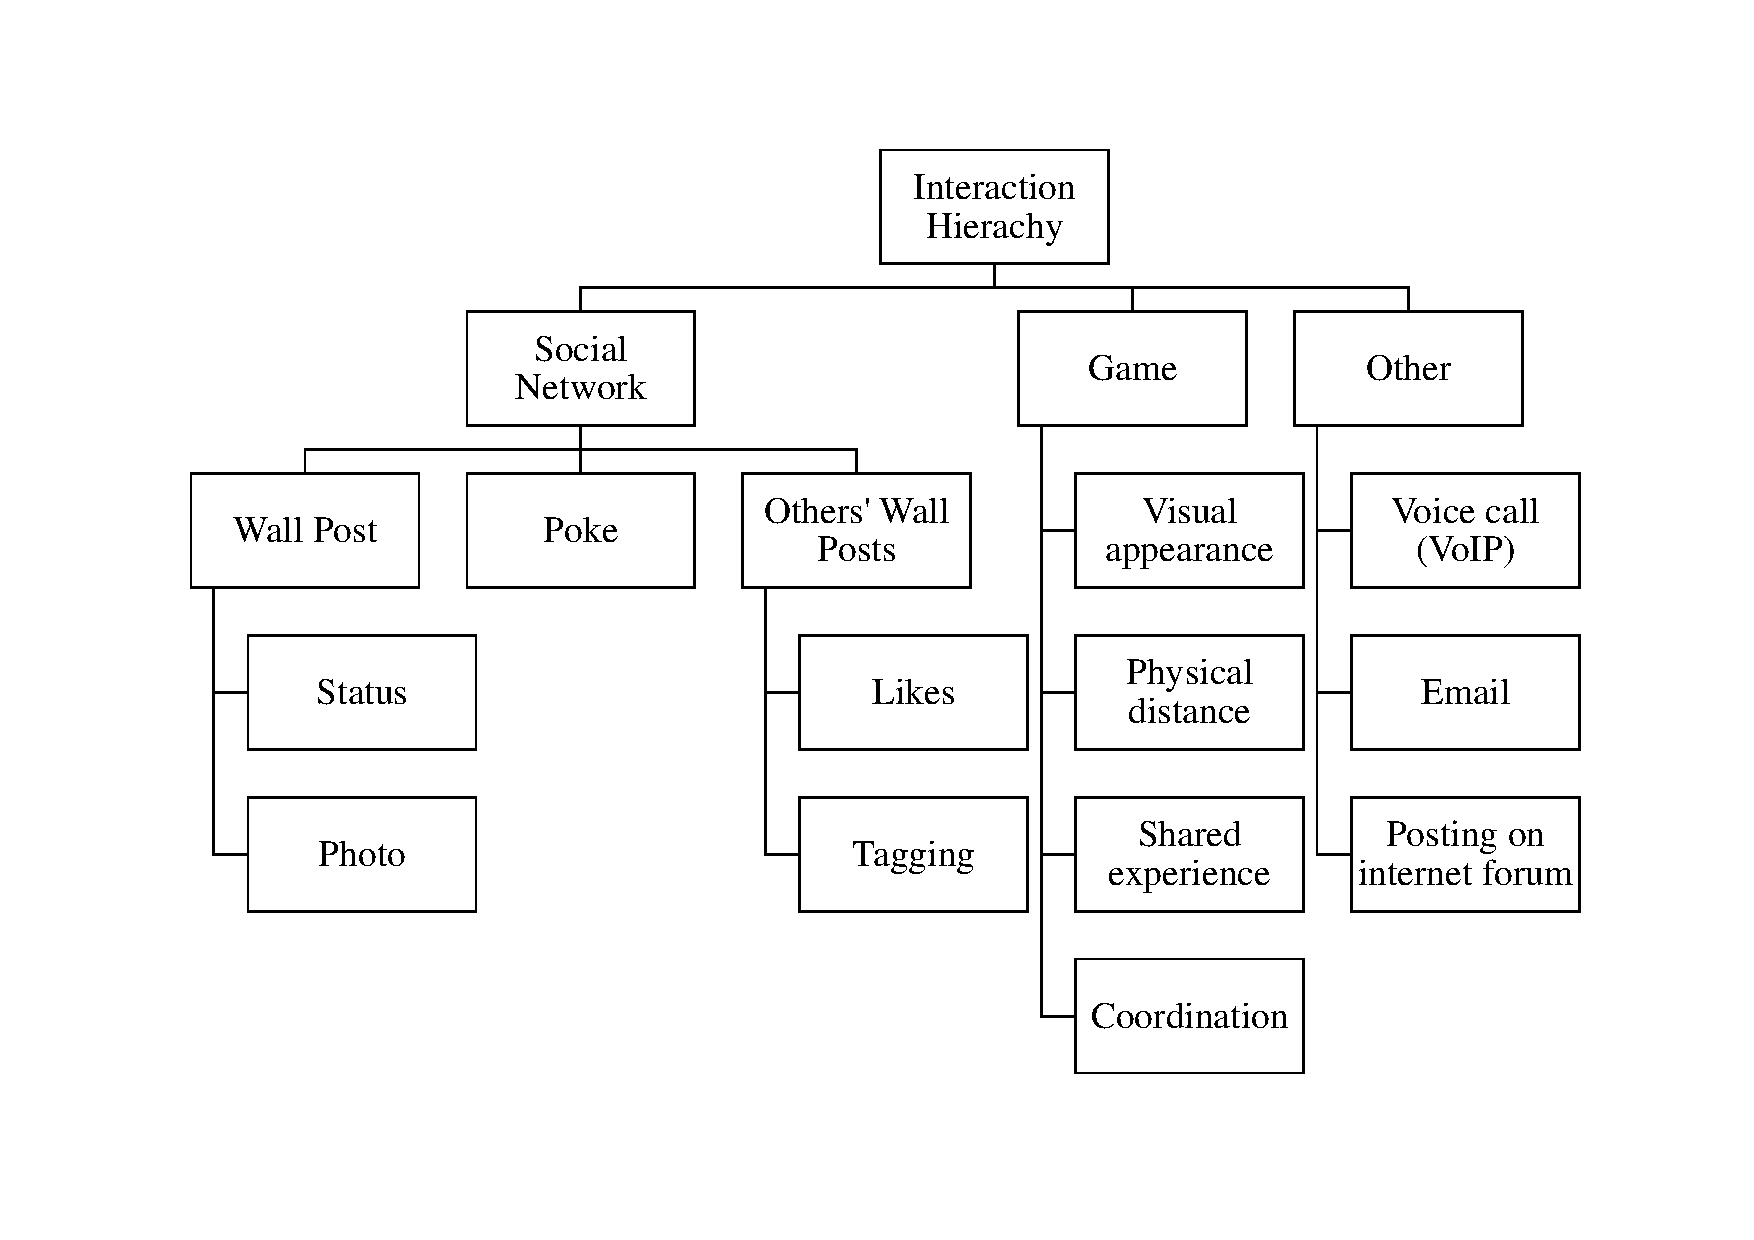
\includegraphics[width=6in]{InteractionTypes.pdf}
\end{center}\end{figure}

\begin{figure}[htb]
\begin{center}
\caption{Interaction Modes}
\label{fig:modes}
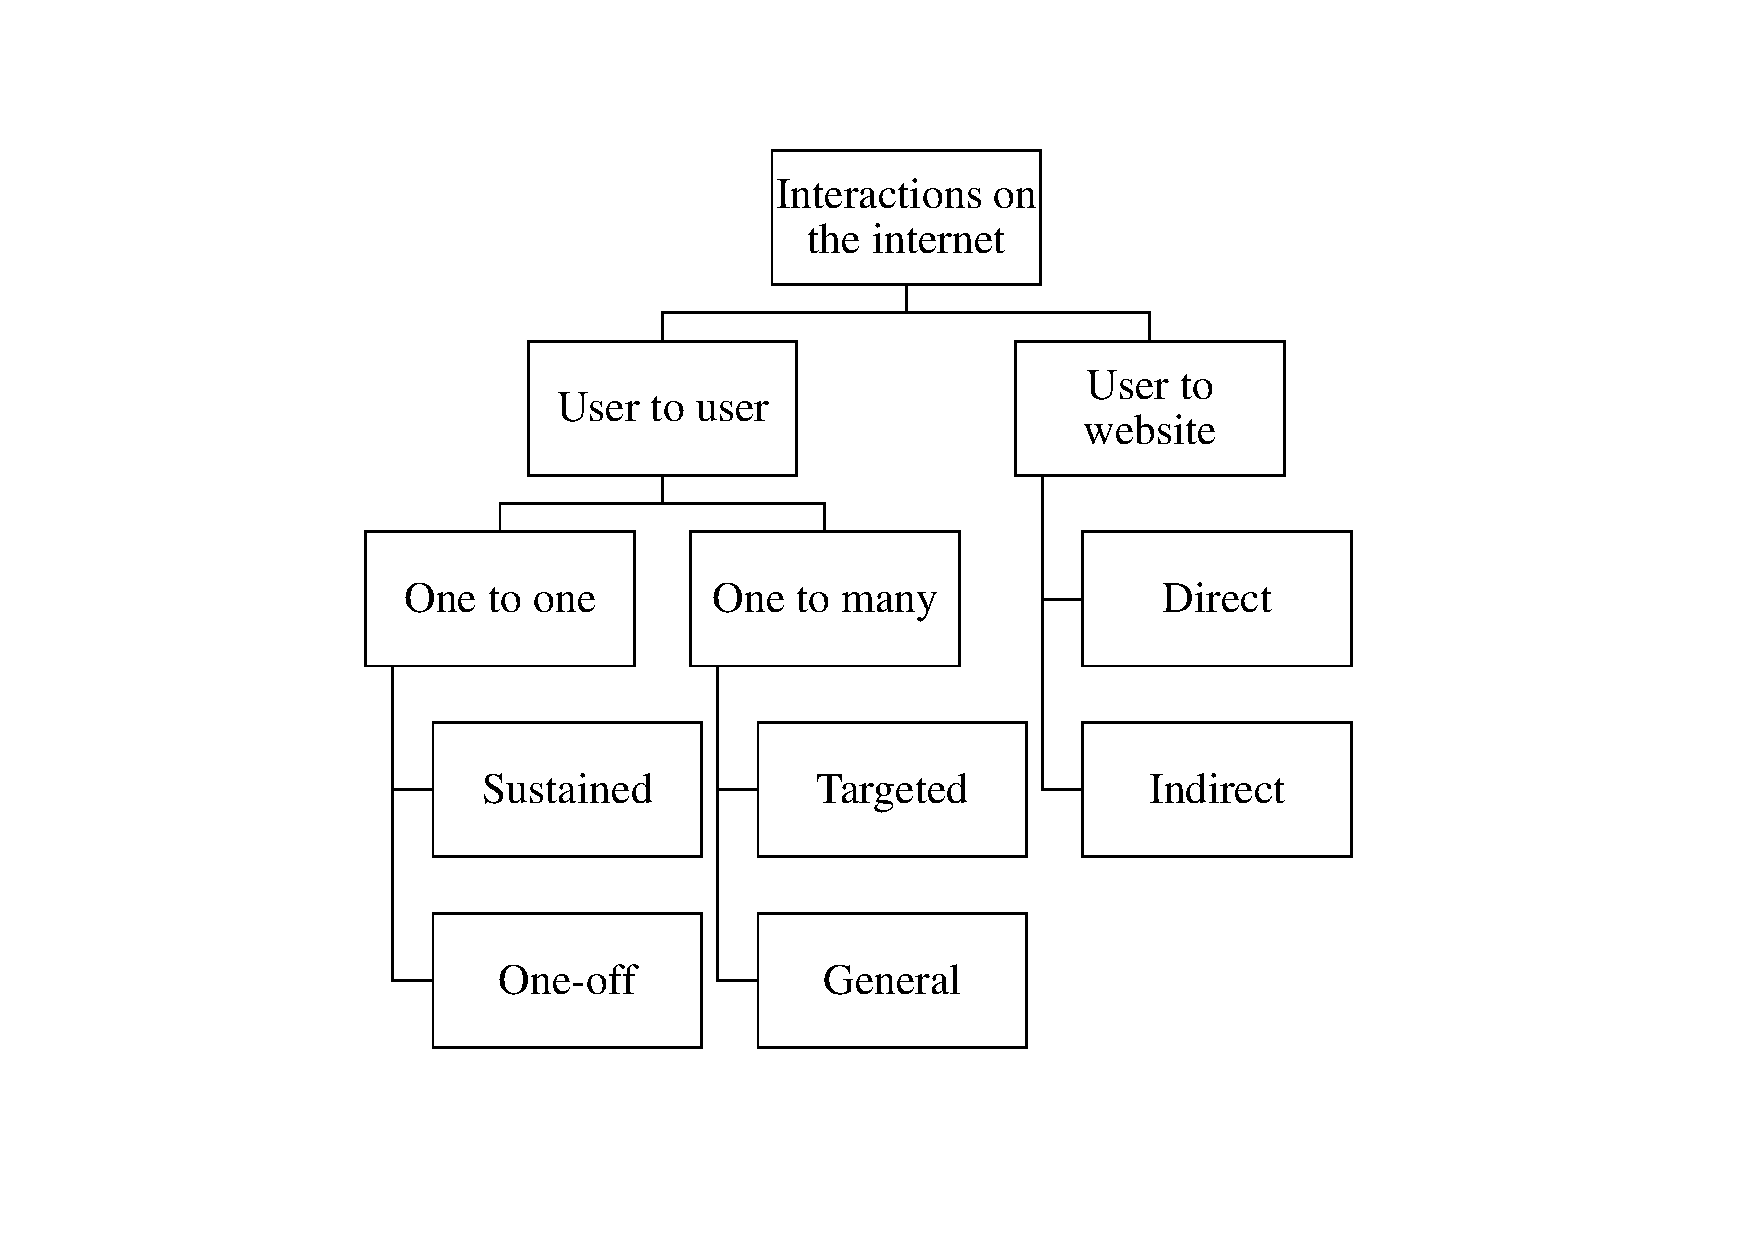
\includegraphics[width=4in]{CategorisationsInteractions}
\end{center}
\end{figure}

When considering multiple modes of interaction I found that there was little current literature linking interaction modes with categorisations. This lead me to then design two hierarchies. The first in order to categorise what different interactions were possible within the virtual environments I was considering, the second to categorise them in terms of how they could be represented.

Initially I produced Figure \ref{fig:types} in order to categorise the types of interactions that were possible. These came largely from personal experience and I produced this in order to help me consider what categories of interactions it would be necessary to visualise. Of course this is not exhaustive but it provided a useful starting point in considering what I would need to categorise.

This lead me to Figure \ref{fig:modes}, which are the modes of interaction that I will be visualising. The model will then be expanded to cover as many of these as possible. These will allow me to experiment both with different visualisations for each of the different modes of interaction and also with the different effects that these will have on the changes of relationships over time and the clustering this causes.

\subsubsection{Requirement 4}
I will implement a way of either importing data downloaded from my or other people's social networks and other sources of relationship data. I will also determine realistic parameters for the generation of my own relationship data that as closely as possible mimics what would be expected from a real person.

\subsubsection{Requirement 5}
The model will evolve in two ways, firstly the people will move around in their 3D environment. A model will be developed to make their motion random but they will not be able to move out of set bounds.

The second way that the model will evolve is in the change in relationships between the pairs of users. This will be affected by the interactions between users within the same environment through the nodes I have detailed above and will also include a decay over time for users who do not interact for more than a certain period of time.

\subsubsection{Requirement 6}
The model will be designed in such a way that the interactions over time will cause relationships between the users to change. This will in turn mean that the users cluster themselves according to their interactions and their starting states. A suitable algorithm will be devised that is able to identify these clusters.

\subsubsection{Requirement 7}
The system will enable a visualisation of the clustering of users and the way that this clustering changes over time. This should be able to be configured by the user to allow clustering according to different metrics and at different levels. This visualisation should also allow the user to see how clustering has changed over time as the model evolves.

\subsubsection{Requirement 8}
The system should output quantitative data about the clustering and evolution of the model over time which can be given real-world applications. Algorithms must be found which can represent the system at different times and which can then take these snapshots and provide meaningful information about the changes between these snapshots.

\subsection{Architecture}

\begin{figure}[htb]
\begin{center}
\caption{Design Pattern Diagram}
\label{fig:pattern}
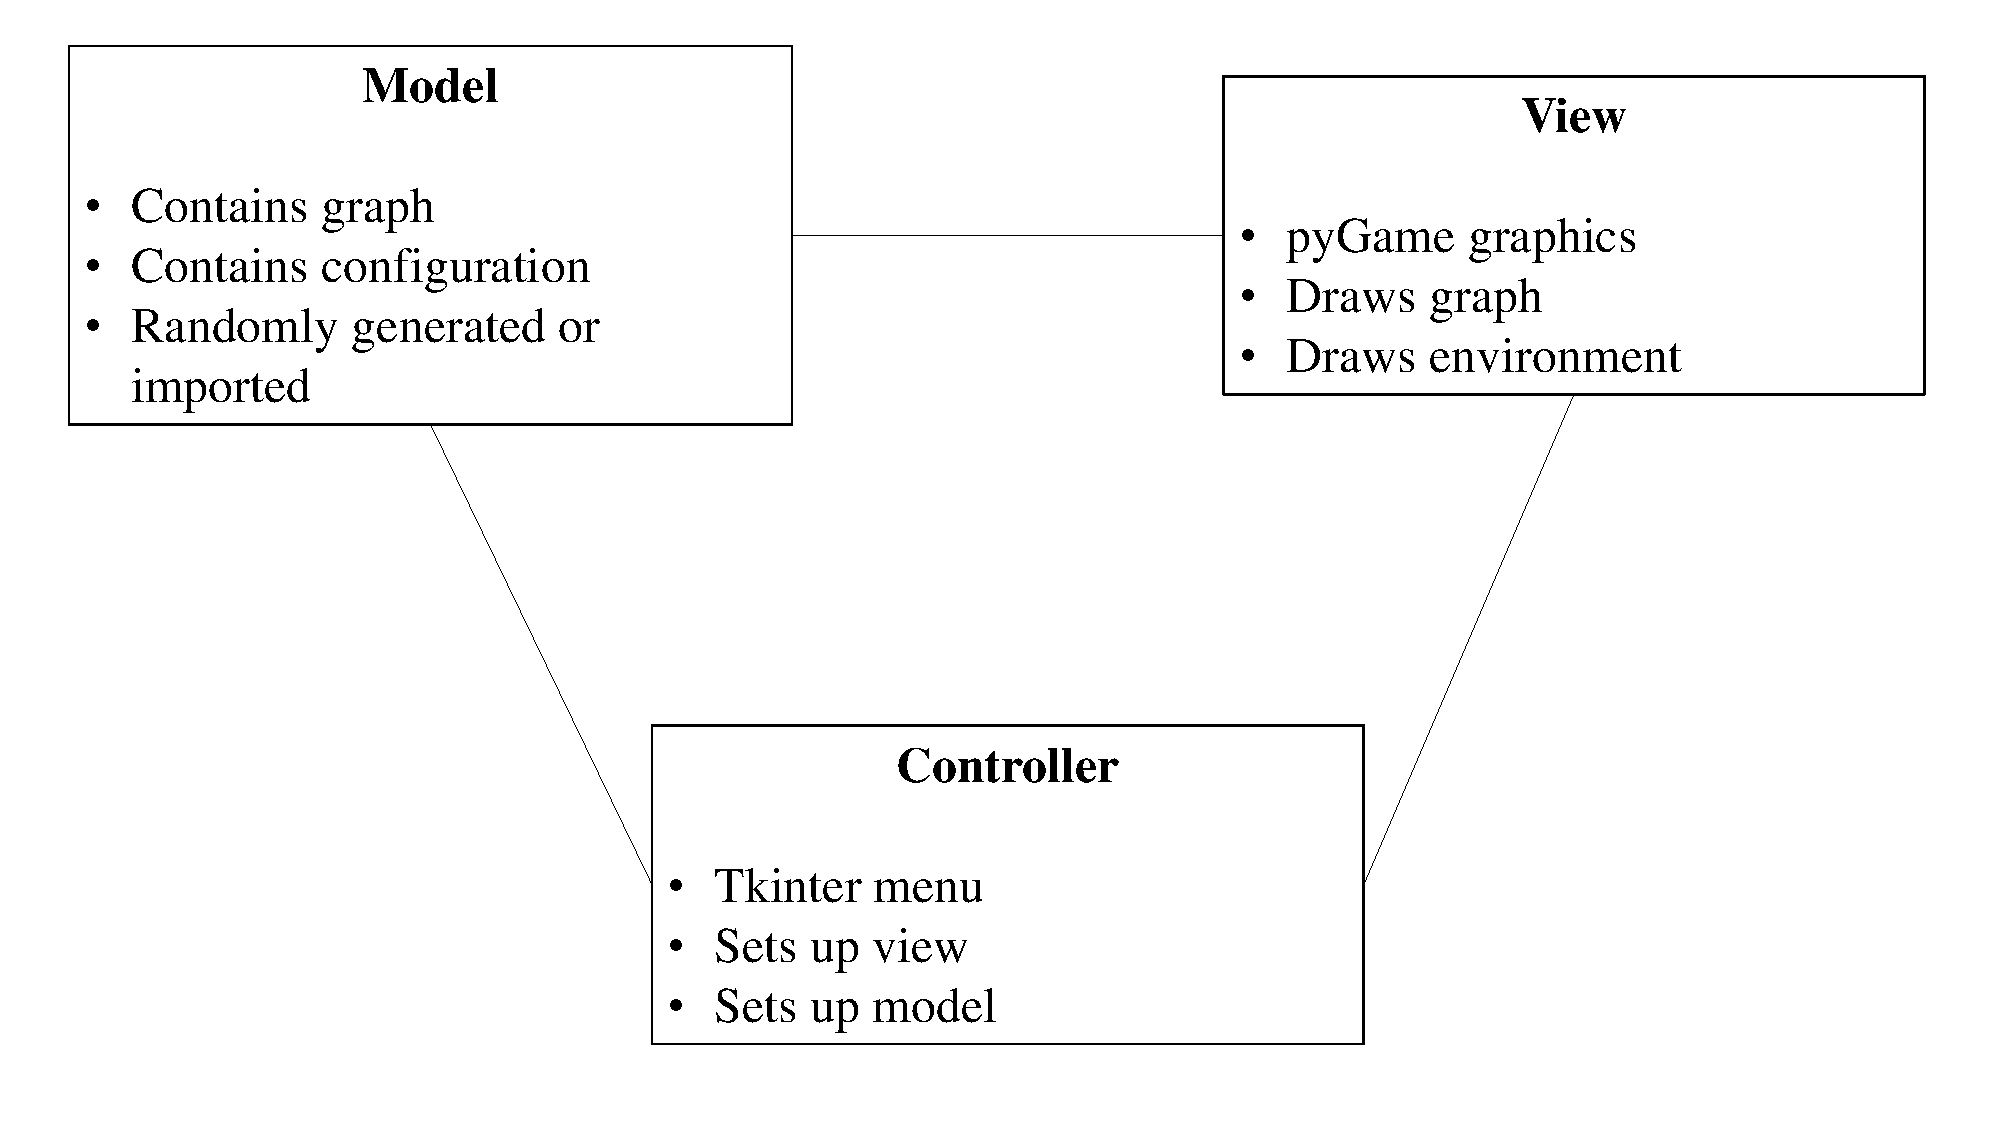
\includegraphics[width=6in]{MVC}
\end{center}
\end{figure}

My design is based on the concept of Model-View-Controller where the core components of my application are split between the model, storing the current state of the system, the view which displays the current state of the system and the controller, which is used the control the state of the system as well as the view. This can be illustrated as in Figure \ref{fig:pattern}. I will now expand on each individual component below.

\subsubsection{Model}
This section will contain the data for the project as well as the means of processing that data and the configuration as a series of classes which can be instantiated as necessary as new data is created or entered.

The most important thing that this part of the model will contain will be the graph. This will either be able to be imported from existing data or generated randomly. In order to import the graph a series of people will have to be specified along with their various attributes in JSON along with a series of relationships between those people. These will then be stored inside people and relationship objects which in turn reside inside a graph object. Alternatively these can be randomly generated to produce a different graph each time with different levels of connectedness.

The model will also store configuration data which will include which elements of the model are to be displayed in which ways, for example the age of a person might be represented by their colour, or it might by the size of their node. This will also store information about the system on which the application is running so that the drawing can be done at an appropriate resolution.

Finally the model will also be responsible for running algorithms in order to evolve the model over time according to the pre-determined rules after each visualisation. The necessary implementation for the analysis of the graph at pre-determined points in order to identify the clustering and the time evolution of the graph will also reside here.

\subsubsection{View}
\begin{figure}[htb]
\begin{center}
\caption{An example visualisation}
\label{fig:visualexample}
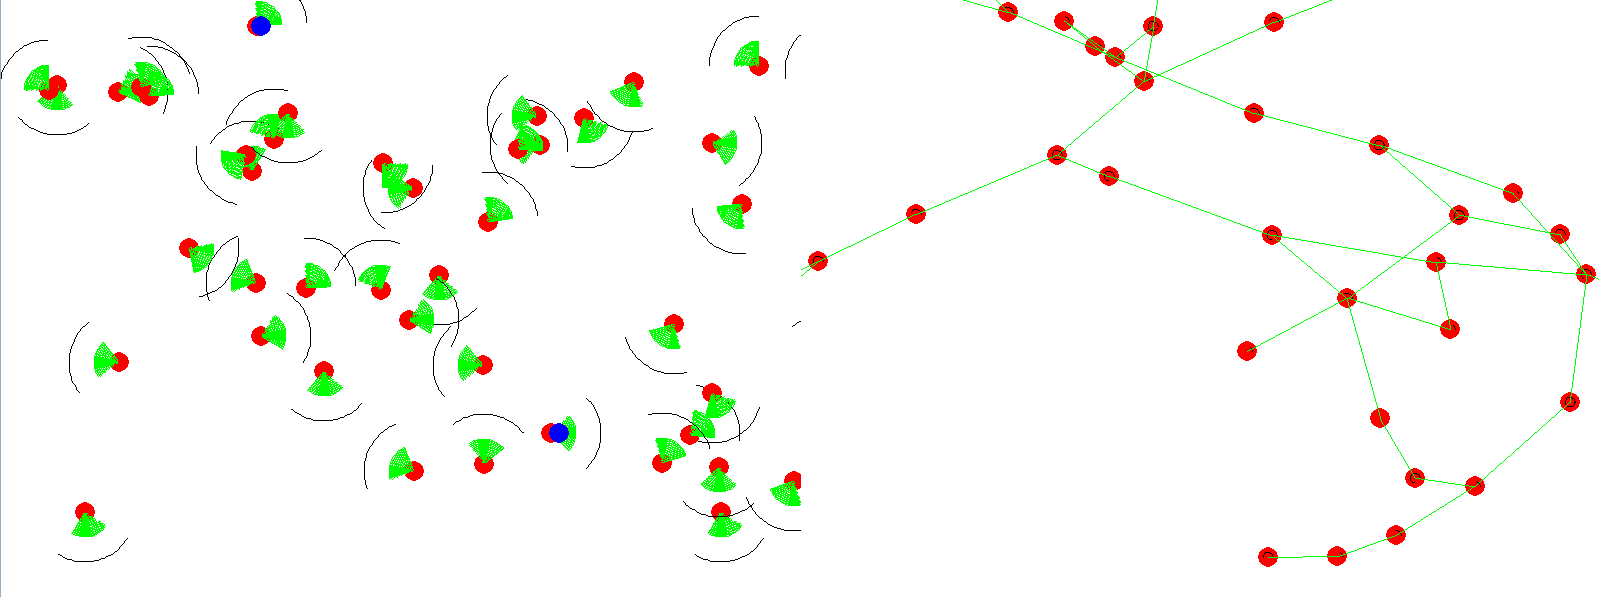
\includegraphics[width=6in]{screen.png}
\end{center}
\end{figure}

This section of the pattern will be responsible for drawing the model at the request of the controller. It will contain classes for both drawing a view of the current relationships as a graph and the current physical locations of the people with various attributes displayed as properties of the visualisation as requested by the controller and specified in the model. As well as this it will also be responsible for visualisations of interactions between the users, as well as their states.

In Figure \ref{fig:visualexample} I have included an example of what the visual output might look like. Here we can see on the right the graph of the relationships between the people and on the other the people's position in the three dimensional environment. In this case the green lines connecting people in the graph represent those with a relationship above a certain strength and the arcs around the circles on the left represent a field of view. We can also see that the graph has a layout according to a force-directed spring algorithm, ensuring that it fits well within the space and that nodes are spread out where possible.

I will develop a system of distorting the presentation based on a Gaussian curve
\begin{equation}
f(x,\mu,\sigma)=\frac{1}{\sigma\sqrt{2\pi}}e^{-\frac{(x-\mu)^2}{2\sigma^2}}.
\end{equation}
where the displacement will depend on $f(x,\mu,\sigma)$ where $x$ will be the distance from the area being examined, $\sigma$ will depend on the size of the presentation space and it will be configurable what $\mu$ should be used. This will make it easier for users to study areas of the visual output which might otherwise be too tightly packed or unclear.

\subsubsection{Controller}
\begin{figure}[htb]
\begin{center}
\caption{Menu displayed by controller}
\label{fig:menu}
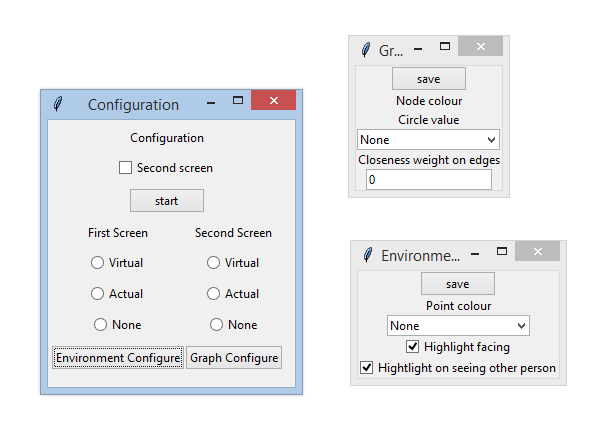
\includegraphics[width=4in]{Config.png}
\end{center}
\end{figure}
The controller will be responsible for configuration of both the model and the view, and starting and ending the whole system. Initially the controller will present a set of menus to the user such as those in Figure \ref{fig:menu}. This will be responsible for the generation of the configuration and then passing it to the model to be used by the view. The controller will then be responsible for ensuring that the view elements draw frames and display them as necessary and for coordinating between the view and the model so that the system is evolved and the clustering measured as necessary.

\subsection{Tools Used}
This project will built using Python 3.4. I chose to use python because it was a language with which I was already familiar and I felt that it would enable to me to quickly develop the necessary model and visualisation. I also believed that the speed of languages such as Java was unnecessary as I planned to produce only two dimensional graphics as output and there was no major computation required for the evolution of the model. The development in python was conducted using the PyCharm IDE which again I was already familiar with and was sell suited to my project.

The graphical output was produced using the PyGame. This was used because it would be easier to use than OpenGL to quickly experiment with different graphical outputs and because it makes used of optimised C code this means that the speed of the graphical output shouldn't slow down any of the computation relating to the model.

The menu was created using the python package Tkinter. I used this as it is the most popular GUI builder for Python and there was already significant documentation available.

Finally I also made use of Numpy. This was used for easier handling of arrays, particularly when calculating positions for layouts of nodes within the graphical output.

\subsection{Development Lifecycle}
I have chosen to use a prototyping model for the development of my software for several reasons. Firstly I wanted the ability to experiment with my system as it was being produced so that I could work out the best way of meeting the requirements I had identified. Secondly I wanted to ensure that what I was producing would work and meet the requirements before the complete system was finished so that if changes needed to be made this could be done earlier in the development process.

The process that I will use will be one of vertical, evolutionary prototypes. Once a suitable base has been developed I will then add complete features individually working towards my requirements. I have chosen this approach because I do not require a complete system to meet my first few requirements and once this is verified as working I can then add additional subsystems to meet the remaining requirements. Evolutionary prototypes will also allow me to refine my design as I go on as I have already selected the tools that I will use for my implementation.

\subsection{Evaluation}
I will evaluate my final system in two ways. First I will spend time comparing my system to other systems that are already available. I will select a number of such systems and compare them by a number of criteria that I will layout below which I believe cover the aims of my project. This will ensure that there is no one system that performs better than mine at my stated goals, even if they do outperform my solution in individual areas.

The criteria that I use will be as follows:
\begin{enumerate}
\item The ability of the system to clearly represent the state of and relationships between people
\item The ability of the system to represent the interactions over different modes between people
\item The ability of the system to represent clustering of the people in the system based on interactions
\item The ability of the system to output quantitative data which can be used to draw useful conclusions regarding the nature of some aspect of the evolution of the model over time
\end{enumerate}

I will then judge this against the following systems:
\begin{description}
\item[Vizster] A project I have already discussed, designed to visualise connections between people in a Friendster network. Available from http://homes.cs.washington.edu/~jheer/projects/vizster/
\item[WolframAlpha Facebook Report] An analysis of data gathered from your Facebook profile by the WolframAlpha website which includes a graphical representation of your friends and gives various indications of the roles friends play in the network. Available from https://www.wolframalpha.com/input/?i=facebook+report
\item[Gephi] This is a tool developed for visualising graphs of all kinds of graph data in very configurable ways. It also supports graphs that evolve over time and allows statistical analysis of graphs. Avaiable from http://gephi.github.io/
\end{description}

Secondly I will measure the extent to which my system is able to solve a real-world problem. My prototyping will enable me to adapt my system to a wide variety of different problems in the field of social network research and so I will be able to look at existing solutions to these problems and compare my solution quantitatively to previous work.

\section{References}

\bibliography{projectpaper}

\end{document}